% Facultad de Ingenier\'ia, Universidad de Buenos Aires
% 75.59 Técnicas de Programación Concurrente I

\documentclass[a4paper,12pt,titlepage]{article}
\usepackage[paperwidth=180mm,paperheight=285mm,left=1.5cm,top=4cm,right=1.5cm,bottom=2cm,head=2.0cm,includefoot]{geometry}
\usepackage[spanish]{babel}
%\usepackage[latin1]{inputenc}
\usepackage[utf8]{inputenc}
\usepackage{lscape}
\usepackage{graphicx}
\usepackage{fancyhdr}
\usepackage{rotating}
%\graphicspath{{../}}

\usepackage{listingsutf8}

\title{75.59 Técnicas de Programación Concurrente I, Trabajo Práctico 2}
\author{Torres, Miguel \and Montoya, Diego \and Garay, Ignacio}

\lhead{
\includegraphics[scale=0.06]{./logo_fiuba.pdf}}
\chead{ 75.59 Técnicas de Programación Concurrente I }
\rhead{}

\lfoot{Garay - Montoya - Torres}
\rfoot{\thepage}
\cfoot{$2^{do}$ Cuatrimestre 2013}

\begin{document}

\thispagestyle{empty}
% T\'itulo del documento.
\begin{center}

\includegraphics{./logo-fiuba.png}\\
\vspace{1cm}
\textsc{\LARGE Universidad de Buenos Aires}\\[0.3cm]
\textsc{\LARGE Facultad de Ingenier\'ia}\\[1.2cm]
\textsc{\Large 75.59 - Técnicas de Programación Concurrente I}\\[0.3cm]
\end{center}

\begin{flushright}
{\large
Montoya, Diego -- 91939\\
Torres, Miguel -- 91396\\
Garay, Ignacio -- 92265\\
\vspace{2cm}
$2^{do}$ cuatrimestre de 2013}
\end{flushright}

\pagestyle{fancy}
\setcounter{page}{1}
\newpage

\tableofcontents
\newpage

\footnotesize
\section{Análisis}
En el análisis del trabajo se identificaron las siguientes identidades del dominio:\\
\begin{itemize}
\item Cliente
\item Servidor
\item Recibidor de Clientes
\item Resolvedor de Paquetes\\
\end{itemize} 

El Servidor es la clase que inicia todos los recursos necesarios para una tener una conversación, creando además
al Recibidor de Clientes y al Resolvedor de Paquetes. El Servidor además es el encargado de de gestionar las 
conversaciones, permitiendo agregar nuevas y administrando las ya existentes.

Cuando un Cliente es iniciado, es el Recibidor de Clientes es el encargado de capturar la solicitud de inicio de sesión para luego comunicarsela al Resolvedor, 
dejando todo listo para que el Cliente pueda crear una nueva conversación o unirse a una existente.

Una vez que algunos clientes forman parte de la misma conversación, los mensajes entre ellos enviados son capturados
por un Receptor de Mensajes perteneciente a cada cliente, el cual se encarga de enviar dichos mensajes al Resolvedor y este los distribuye a las conversaciones correspondientes.

Puede verse entonces que el Cliente actúa como productor de mensajes, los cuales son consumidos por el Receptor de Mensajes y este a la vez es un productor de paquetes que estos son consumidos por el Resolvedor.\\

\subsection{Casos de Uso}
Se identificaron además los siguientes casos de uso, desde el punto de vista del usuario:\\
\begin{figure}[h!]
\centering
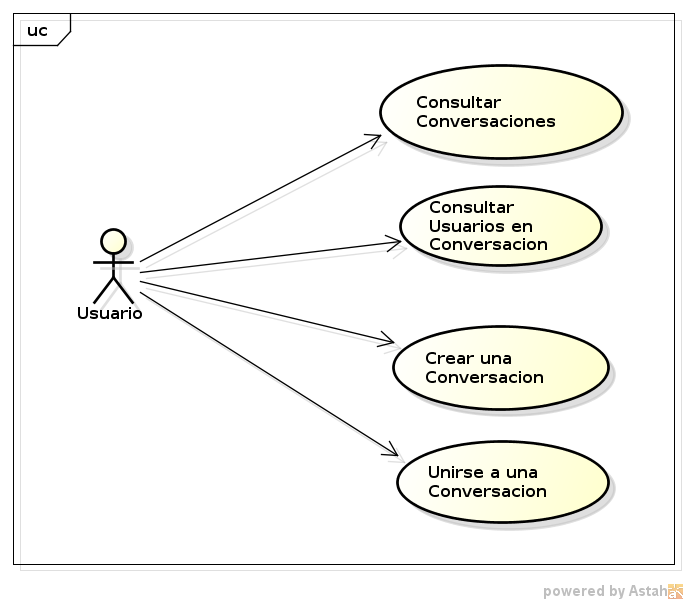
\includegraphics[width=0.6\textwidth]{CasosDeUso2.png}
\caption{Diagrama de casos de uso del Cliente}
\label{fig:casos_uso}
\end{figure}

\begin{itemize}
\item \textbf{Consultar conversaciones}\\
  Es el caso de uso en el cual el Cliente conectado al Servidor decide realizar una consulta sobre las conversaciones
  existentes actualmente en el Servidor.
\item \textbf{Consultar Usuarios en Conversacion}\\ 
  Es el caso de uso en el cual un Cliente conectado al Servidor solicita ver un listado de los usuarios que se encuentran dentro de una conversacion especifica.
\item \textbf{Crear una conversación}\\ 
  Es el caso de uso en el cual un Cliente conectado al Servidor decide iniciar una nueva conversación, en la cual inicialmente
  será el único miembro, hasta que otro Cliente decida unirse para conversar.
\item \textbf{Unirse a una conversación}\\
  Es el caso de uso en el cual un Cliente luego de consultar las conversaciones existentes en el Servidor decide además
  unirse a una de ellas.\\
\end{itemize} 


\newpage
\section{Diseño}

Para la resolución de la concurrencia en la aplicacion se implementaron varias herramientas como Fifo, Pipe, Lock , 
Memoria Compartida, Señales y Sockets.

Se creó un proceso encargado de la generacion de los recursos y administración de las conversaciones, llamado 
appServidor, el cual es el punto de inicio de la aplicación.\\

También existe el proceso llamado appCliente, el cual es creado cuando un usuario inicia un Cliente y le permite interactuar con
el Servidor para unirse a una conversación o iniciar una nueva\\

\subsection{Servidor}
Dentro del proceso appServidor se crean 2 nuevos procesos llamados Resolvedor y Recibidor que se encargar de resolver todas la solicitudes 
y recibir nuevos clientes respectivamente.
El funcionamiento del servidor es el siguiente, cuando un cliente intenta conectarse, éste le envia un paquete de inicio de sesión (a traves 
de una conexion UDP), este paquete es captado por el proceso Recibidor, quien crea un nuevo proceso Receptor para ese cliente, luego 
se retransmitirá el paquete y algunos datos más de conexión al proceso Resolvedor y al nuevo Receptor (utilizando un area de memoria compartida). 
Luego el recibidor espera una confirmacion (mediante un semáforo) del proceso Receptor para poder seguir escuchando nuevos usuarios.\\

La tarea que lleva a cabo el proceso Resolvedor es almacenar todos los usuarios en linea, todas las conversaciones abiertas y de reenviar 
todos los mensajes que se envien entre si. Para ello cuando arriba un paquete a la Cola de Paquetes (un area de memoria compartida para colocar 
los paquetes de los usuarios que iniciaron sesión) éste lo retira de allí, verifica qué tipo de paquete es, resuelve la petición correspondiente y 
le envía la respuesta al usuario o a todos los integrantes dentro de una conversación si se tratase de un mensaje. Este procedimiento se repite 
hasta que el proceso padre le envie una señal de finalización.\\

El proceso Recibidor se encarga de escuchar conexiones entrantes de nuevos usuarios. Cuando un nuevo usuario 
desea conectarse, el proceso recibe una solicitud de conexion mediante un paquete, lo primero que hace es lanzar un proceso Receptor que atendera los mensajes enviados por ese cliente(al lanzarlo espera que inicie correctamente para continuar), luego crea un nuevo paquete de inicio de sesion con la informacion del usuario y lo inserta en la Cola de Paquete, para que se encargue el Resolvedor.\\

Cuando llega una solicitud de inicio de sesión al Resolvedor, éste es informado cuando retira un paquete de la Cola de Paquetes con el tipo PROTO\_INICIO\_SESION que es fue insertado por el proceso
Recibidor. La tarea que se lleva el a cabo el Resolvedor es la siguiente, se lee la información de usuario (direccion de socket, pid del proceso receptor y nombre), se comprueba de que no exista otro usario con el mismo nombre, se lo agrega y se le envia una señal para que continue normalmente al proceso Receptor asociado al cliente, en caso contrario (ya existe otro usuario con el mismo nombre) se le indica al mismo proceso Receptor que le indique la situacion al cliente y finalice.
 Luego de realizar todo esto el proceso Resolvedor se dispone a retirar otro paquete de la Cola si es que huberia o bloqueandose sino.\\

La tarea basica de cada proceso Receptor instanciado es colocar los paquetes que reciba por parte de un cliente y los coloque dentro de la Cola De Paquetes. Su ejecucion finaliza cuando el usuario a cargo decide finalizar la sesion o si el Servidor decide cerrarse (siendo esta situacion informada por parte del recibidor mediante una señal de finalizacion).

\subsection{Paquete}
Los paquetes utilizados en toda la aplicación se diseñaron para resolver varios problemas (como iniciar y finalizar sesión, crear y unirse a una 
conversación, mensajes, etc) y así resolverlos todos contenidos en una misma estructura.
Se pensaron para que sean de tamaño fijo, de 512 bytes concretamente, conformando la siguiente estructura:

\begin{itemize}
\item Cabecera: 2 bytes en formato Big Endian para el tamanio del paquete, 1 byte para el tipo de paquete y 1 ultimo byte para la cantidad de atributos.
\item Datos: 508 bytes disponibles para datos, en donde se almacenaran los atributos del paquete.\\
\end{itemize}

Según el tipo de paquete que sea se resuelve una solicitud diferente. Los diferentes tipos de paquetes son los siguientes:
\begin{itemize}
\item PROTO\_INICIO\_SESION: indica que un usuario intenta iniciar sesion, solo usado dentro del servidor.
\item INICIO\_SESION: indica que un usuario intenta inciar sesion.
\item FIN\_SESION: indica que un usuario desea finalizar su sesion.
\item MENSAJE: contiene el mensaje que envio un usuario, en la conversacion donde se encuentra.
\item CREAR\_CONVERSACION: indica que un usuario quiere crear una converasacion.
\item UNIRSE\_CONVERSACION indica que un usuario desea unirse a una conversacion ya creada.
\item CONVERSACIONES: indica una solicitud para que ver las conversaciones disponibles.
\item USUARIOS\_CONVERSACION: indica una solicitud para que ver los usuarios dentro de una conversacion.
\item USUARIOS\_EN\_LINEA: indica una solicitud para que ver todos los usuarios que se encuentran conectados.
\item OK: indica una confirmación sobre algún evento por parte del servidor (inicio y fin de sesion, etc).
\item ERROR: indica un error ocurrido cuando se proceso una solitud de un usuario.
\item SERVIDOR\_CERRADO: indica que el servidor termino su ejecucion o fue cerrado.
\item DESCONOCIDO: identifica al paquete como desconocido y no se lo puede procesar.\\
\end{itemize}

\subsection{Sistema de Log}

Se implemento el mismo sistema de log que en primer proyecto, el cual divide los sucesos en diferentes categorías, las cuales son:
\begin{itemize}
\item Info: informacion corriente de los pasos de la ejecucion.
\item Debug: informacion de debug.
\item Fatal: indica una excepcion lanzada.
\item Warning: informacion de advertencia sobre algun comportamiento anormal.
\item Error: indica un error critico en la aplicacion
\end{itemize}
El archivo de salida de Log esta resguardado por un Lock para su correcta escritura por los distintos procesos que vuelcan su información.

\newpage
\section{Diagramas}
\subsection{Diagrama de Comunicacion}
En el siguiente diagrama se puede ver como es la forma comunicaion de un usuario con la ya dentro de una conversacion, enviando y recibiendo mensajes.
\begin{figure}[h!]
\centering
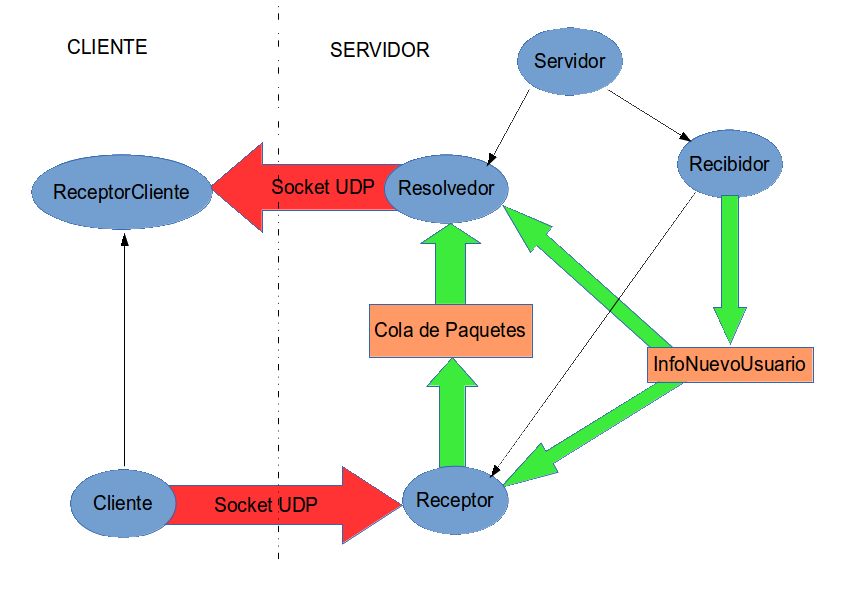
\includegraphics[width=0.8\textwidth]{dia_comunicacion.png}
\caption{Diagrama de comunicacion entre procesos}
\label{fig:comunicacion}
\end{figure}

\newpage
\subsection{Diagrama de Clases}
Diagrama de clases con Objetos mas importantes del Servidor, solo hay un objeto Singleton por proceso, describiendo la relacion con los otros objetos utilizados para la comunicacion entre ellos. 
\begin{figure}[h!]
\centering
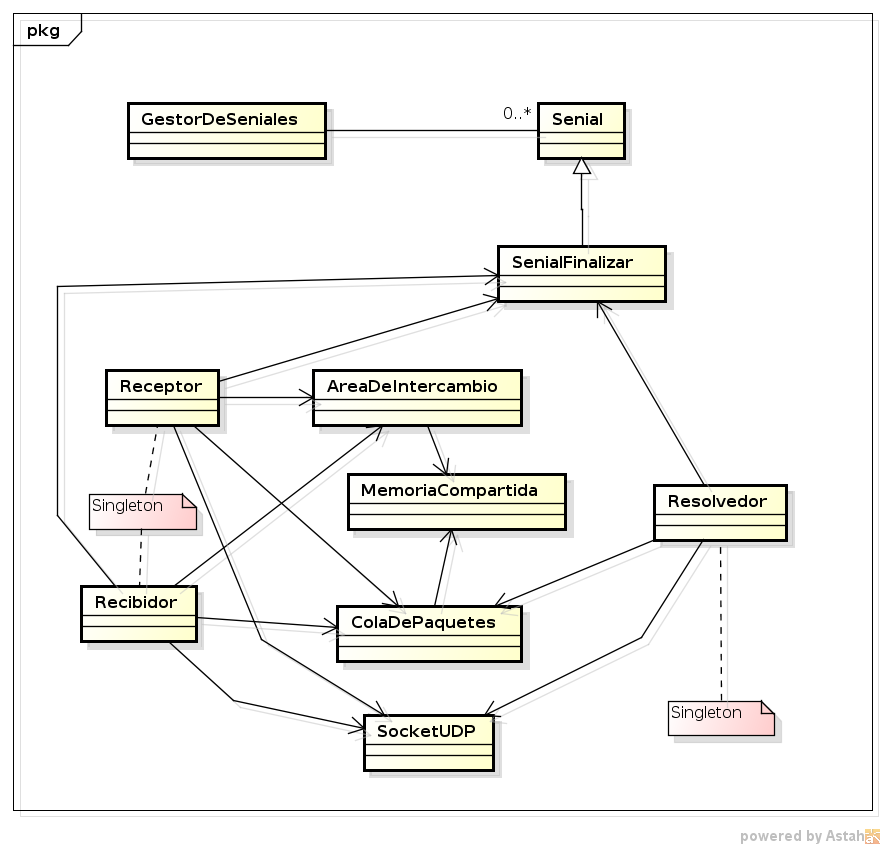
\includegraphics[width=0.8\textwidth]{dia_clases-servidor.png}
\caption{Diagrama de clases del Servidor con los mecanismos IPCs más representativos}
\label{fig:clases}
\end{figure}

El diagrama de clases de un cliente no es relevante ya que solo constaria de una unica clase.

\subsection{Diagrama de Estados}
Diagrama de transcion de estados para un cliente.
\begin{figure}[h!]
\centering
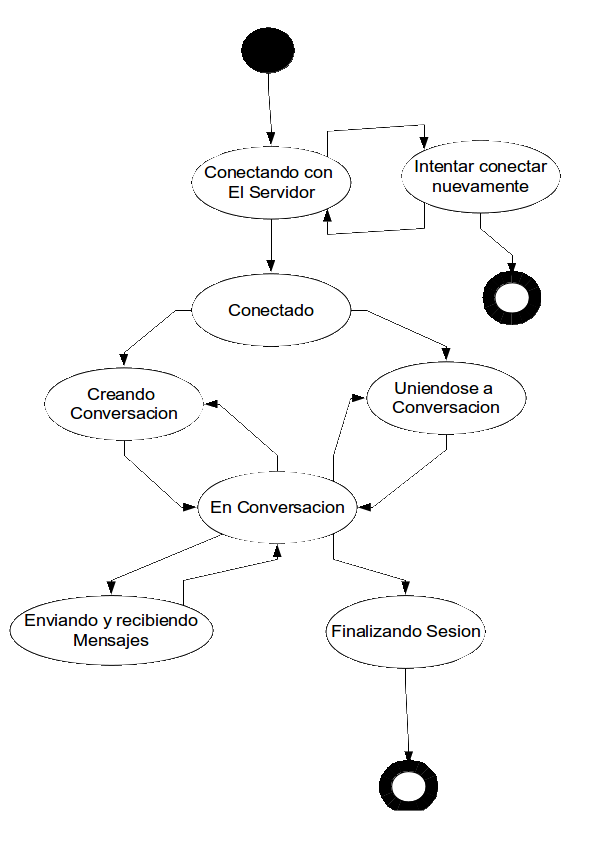
\includegraphics[width=0.7\textwidth]{dia_estados_cliente.png}
\caption{Diagrama de Estados de un cliente.}
\label{fig:estados}
\end{figure}

\newpage
\section{Integración}
\subsection{Intercambio de Informacion}

Para la recibir los mensajes de los distintos usuarios se implemento una Cola de Paquetes que utiliza internamente un segmento de 
Memoria Compartida y 3 semaforos (uno para sacar, otro para insertar y otro para leer/escribir del segmento de memoria). Esta Cola es 
instanciada por el proceso Resolvedor y por todos los procesos Receptor (1 por cada usuario en conectado).\\

Para enviar la informacion de un nuevo usuario a los otros procesos por parte del Recibidor se implemento una clase llamada AreaDeIntercambio 
que utiliza un segmento de memoria compartida en donde se guarda informacion del nuevo usuario, como el nombre del nuevo usuario, el PID del 
proceso Receptor que gestionara los paquetes enviados por ese usuario y datos sobre la direccion UDP del socket del cliente.\\

\subsection{Sincronización}

Para sincronizar entre todos los procesos involucrados en el inicio de sesion de un nuevo usuario se utilizaron semaforos. Un semaforo es utilizado 
por el Resolvedor cuando este modifica sus estrucutas internas y al momento de enviar los paquetes de respuesta a los distintos usuarios, por lo 
que antes de enviar la señal de un nuevo usuario el recibidor hace un wait() del semaforo para asegurar que no pongo en riesgo ningun elemento interno 
del resolvedor. Otro semaforo es utilizado por el un Receptor y el Recibidor al momento de crear un nuevo usuario donde el wait() lo hace el Recibidor 
esperando que inicie correctamente el Receptor y se quede en estado de espera para la confirmacion de continuar(en caso de positivo o negativo del inicio 
de sesion del usuario). Cuando el Receptor recibe la confirmacion de continuar, para ambos escenarios(inicio correctamente sesion o se produjo un error) se le indica la situacion al usuario y continua a la espere de recibir mensajes del cliente o finaliza segun el caso.\\

Para sincronizar la correcta finalizacion de todos los procesos se implemento una Señal llamada SenialFinalizar, que establece la condicion de corte del bucle de ejecucion para un proceso. Las condiciones de corte para la mayoria de los procesos se utilizaron booleanos, para el Resolvedor es seguirEnviando, para el Recibidor es seguirEscuchando y para cada Receptor es seguirRecibiendo. Cuando un proceso recibe una señal de finalizar, el manejador de la señal establece en FALSE el booleano de control.

\subsection{Cliente}
Un cliente solo consta de dos procesos(una vez establecida la conexion con el servidor) donde uno se encargar de enviar paquetes y el otro recibir las respuestas. 
El emisor envia paquetes segun lo ingresado por entrada estandar y el receptor imprime por salida estadar los paquetes que le llegan.

\end{document}

